\documentclass[10pt]{beamer}
\usepackage[utf8x]{inputenc}
\usepackage{hyperref}
\usepackage{fontawesome}
\usepackage{graphicx}
\usepackage[english,ngerman]{babel}
\graphicspath{ {./images/} }
% ------------------------------------------------------------------------------
% Use the beautiful metropolis beamer template
% ------------------------------------------------------------------------------
\usepackage[T1]{fontenc}
\usepackage{fontawesome}
\usepackage{FiraSans} 
\mode<presentation>
{
  \usetheme[progressbar=foot,numbering=fraction,background=light]{metropolis} 
  \usecolortheme{crane} % or try albatross, beaver, crane, ...
  \usefonttheme{structurebold}  % or try serif, structurebold, ...
  \setbeamertemplate{navigation symbols}{}
  \setbeamertemplate{caption}[numbered]
  %\setbeamertemplate{frame footer}{My custom footer}
} 

% ------------------------------------------------------------------------------
% beamer doesn't have texttt defined, but I usually want it anyway
% ------------------------------------------------------------------------------
\let\textttorig\texttt
\renewcommand<>{\texttt}[1]{%
  \only#2{\textttorig{#1}}%
}

% ------------------------------------------------------------------------------
% minted
% ------------------------------------------------------------------------------
\usepackage{minted}


% ------------------------------------------------------------------------------
% tcolorbox / tcblisting
% ------------------------------------------------------------------------------
\usepackage{xcolor}
\definecolor{codecolor}{HTML}{FFC300}

\usepackage{tcolorbox}
\tcbuselibrary{most,listingsutf8,minted}

\tcbset{tcbox width=auto,left=1mm,top=1mm,bottom=1mm,
right=1mm,boxsep=1mm,middle=1pt}

\newtcblisting{myr}[1]{colback=codecolor!5,colframe=codecolor!80!black,listing only, 
minted options={numbers=left, style=tcblatex,fontsize=\tiny,breaklines,autogobble,linenos,numbersep=3mm},
left=5mm,enhanced,
title=#1, fonttitle=\bfseries,
listing engine=minted,minted language=r}


% ------------------------------------------------------------------------------
% Listings
% ------------------------------------------------------------------------------
\definecolor{mygreen}{HTML}{37980D}
\definecolor{myblue}{HTML}{0D089F}
\definecolor{myred}{HTML}{98290D}

\usepackage{listings}

% the following is optional to configure custom highlighting
\lstdefinelanguage{XML}
{
  morestring=[b]",
  morecomment=[s]{<!--}{-->},
  morestring=[s]{>}{<},
  morekeywords={ref,xmlns,version,type,canonicalRef,metr,real,target}% list your attributes here
}

\lstdefinestyle{myxml}{
language=XML,
showspaces=false,
showtabs=false,
basicstyle=\ttfamily,
columns=fullflexible,
breaklines=true,
showstringspaces=false,
breakatwhitespace=true,
escapeinside={(*@}{@*)},
basicstyle=\color{mygreen}\ttfamily,%\footnotesize,
stringstyle=\color{myred},
commentstyle=\color{myblue}\upshape,
keywordstyle=\color{myblue}\bfseries,
}

% ------------------------------------------------------------------------------
% The Document
% ------------------------------------------------------------------------------
\title{ECS in Game Development}
\author{Jorge Pinto Sousa (He/Him), Luiz Jardim (Viceroy/Viceroyer)}

\institute{Critical Techworks}
\date{July 2021}
\usemintedstyle[yaml]{}
\newcommand{\cpp}{C++}
\newcommand\myheading[1]{%
  \par\bigskip
  {\Large\bfseries#1}\par\smallskip}



\begin{document}

\begin{frame}
\titlepage
\end{frame}

\section{Entity–component–system (ECS)}
\begin{frame}[fragile]{Entity–component–system (ECS)}
    \begin{center}
        \myheading{\textit{Separate data from behaviour.}}
    \end{center}
\end{frame}
\begin{frame}[fragile]{Entity–component–system (ECS)}

\begin{itemize}
    \item
        It addresses some of the problems with object orientation while promoting code reusability, extendability, maintanability and paralle... para... parallelizability (is this a word?).
    \item 
        One of it's greatest features is easily modifying behaviour at runtime.
\end{itemize}
\end{frame}

\begin{frame}[fragile]{ECS - Characteristics}

ECS has:
\begin{itemize}
    \item   
        \textbf{Entities} are unique "things (identifiers).
    \item
        \textbf{Components} which are just datatypes without \textbf{behaviour}
    \item
        \textbf{Systems} which are functions that will act in \textbf{Entities} that have a certain set of
        \textbf{Components}.

\end{itemize}
\end{frame}

\begin{frame}[fragile]{ECS - Characteristics}

Also:
\begin{itemize}
    \item 
        \textbf{Entities} can contain zero or more \textbf{components}.
    \item 
        \textbf{Entities} can dynamically change \textbf{components}.
\end{itemize}
There are frameworks that implement and enable this design pattern. 

In the scope of this presentation we'll use \href{https://bevyengine.org/}{\color{blue}{Bevy}}.
\end{frame}

\begin{frame}[fragile]{ECS - Characteristics}

Despite the \textit{"by the book"} definition of ECS, which has to have entities, component and systems, sometimes in practice that is not the case.

Usually anything that let's you add stuff to entities and then querying them for those things, are usually considered to be an ECS.

\end{frame}

\begin{frame}[fragile]{ECS is not EC}

In an EC framework, components contain both data and behaviour, and that behaviour is executed directly on the component.

(Place example here)
\end{frame}

\begin{frame}[fragile]{Is ECS too different from OOP?}
\begin{center}
\myheading{Composition over inheritance.}
\end{center}
\end{frame}

\begin{frame}[fragile]{Is ECS too different from OOP?}
\begin{center}
\myheading{Exposed Plain Data Objects over encapsulation.}
\end{center}
\end{frame}

\begin{frame}[fragile]{Is ECS too different from OOP?}
\begin{center}
\myheading{Separate data and behaviour.}
\end{center}
\end{frame}

\begin{frame}[fragile]{Is ECS too different from OOP?}
\begin{center}
\myheading{OOP object instances are of a single non-changing type, while entities can have dynamically changing components.}
\end{center}
\end{frame}

\begin{frame}[fragile]{ECS - An example}
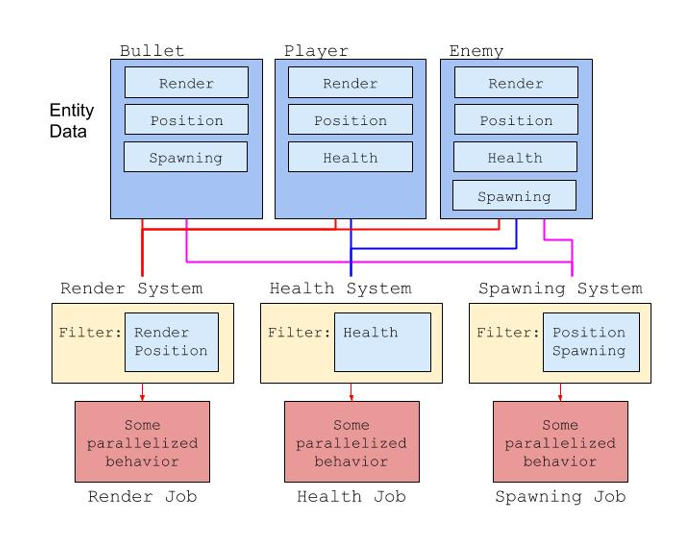
\includegraphics[width=10cm,height=7cm]{../images/image.png}
\end{frame}

\begin{frame}[fragile]{References}
\begin{itemize}
    \item
        \href{https://bevyengine.org/}{\color{blue}{Bevy}}
    \item 
        \href{https://github.com/SanderMertens/ecs-faq}{\color{blue}{ecs-faq}}
    \item
        \href{https://software.intel.com/content/www/us/en/develop/articles/get-started-with-the-unity-entity-component-system-ecs-c-sharp-job-system-and-burst-compiler.html}{\color{blue}{Get Started with the Unity* Entity Component System (ECS)}}
\end{itemize}
\end{frame}
\end{document}
